\section{Moravec}\label{sec:moravec}
Moravecs hjørne detektor\cite{moravec}, er en af de tidligste feature detektorer, og definere et hjørne som værende et område med lav selvlighed. Moravec anvender denne definition til at opnå en matematisk formulering af hjørner ved, for hvert punkt i billedet, at udregne auto-korrelationen af overlappende pixel regioner af 3x3, 5x5 eller 7x7 dataindsamlingsvinduer. En høj auto-korrelation imellem de overlappende pixelregioner vil betyde lav selvlighed og derved et hjørne. Dataindsamlingsvinduet kan derved bruges til at detektere hjørner, ved at forskyde dette med én pixel i alle principielle retninger (horisontalt, vertikalt og diagonalt) og udregne intensitetsvariationen (auto-korrelationen) af alle de forskudte vinduer. Denne variation kan beskrives med en vægtet funktion over vinduet  \emph{(SSD: Summed Square Difference)}, der udregner forskellen på vinduerne:
\begin{equation}
E(u,v)= \sum_{\forall \text{x,y i dataindsamlingsvinduet}} w(x,y)[I(x+u,y+v) - I(x,y)]^2
\label{moravec}     
\end{equation}
hvor $(u,v)\in \lbrace -1,0,1 \rbrace$ er forskydningen af vinduet, der summere over alle pixels i dataindsamlingsvinduet $w$, der har centrum i $(x,y)$. 
Figur \ref{fig:moravec} illustrere en udregning af $SSD$ af et diagonalt skift på en isoleret sort pixel (med en intensitet på 0) på en hvid baggrund (med en intensitet på 255) og på et idealt hjørne. Det røde vindue indikere det originale vindue og det blå indikere  vinduet forskudt med vektoren i retningen $(1,1)$. 
\begin{figure}[H]
    \centering
    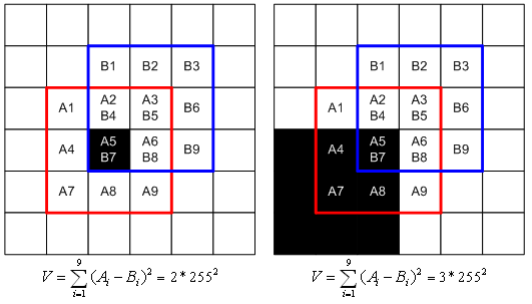
\includegraphics[width=0.55\textwidth]{fig/25.png}
     \vspace{-1em}
    \begin{center}    
       \caption{\textcolor{gray}{\footnotesize \textit{ SSD udregninger for intensitetsvariationer imellem forskudte vindue. }}}
    \label{fig:moravec}
     \end{center}
     \vspace{-2.5em}
  \end{figure} \noindent   
Af de otte skift genereres otte intensitetsvariationer ift. det originale vindue. Den mindste forskel af disse otte variationer, definere punktets \textit{hjørnestyrke}.
$$
C(x,y)=min(E(u,v))
$$
En horisontal kant vil have en stor selvlighed (lav auto-korrelation) med et dataindsamlingsvindue forskudt horisontalt derfor, for at identificere hjørner, tages minimum af $E$ for at sikre en lav selvlighed (stor auto-korrelation) i alle retninger. 
Der opstilles en grænseværdi $t$ for $C$, der bestemmer om punktet er et hjørne(sandt/falsk) og derved om det kan udvælges som et interessepunkt.
\begin{equation}
\begin{split}
\texttt{hjørne} = 
\begin{cases}
\texttt{sandt}& \texttt{hvis } C(x,y)\geq t, \\
\texttt{falsk }& \texttt{hvis } C(x,y) < t.
\end{cases}
\end{split}
\label{cornerind}
\end{equation}
 \\ \\
Moravec lider af følgende problemer pga. dens simplicitet. 
\begin{itemize}
\item{Der undersøges kun et diskret sæt af pixelskift (i hver principiel retning) og resultatet er derfor anisotropisk, (afhængig af retning). Undersøges en kant, der ikke er horisontal, vertikal eller diagonal, vil den mindste intensitetsvariation være stor, og derved kan punktet fejlagtigt detekteres som et hjørne.}
\item{Det skiftende vindue er rektangulært, og metoden er derfor meget følsom overfor støj i billedet.}
\item{Detektoren finder punkter lokaliseret på kanter. Små deformationer i kanterne som støj, vil resultere i at den mindste intensitetsvariation vil være relativt stor, og derfor detektere punktet som værende et interessepunkt.}
\end{itemize}
% <evt konklusion>
% <måske billeder download cornerdetection.pdf>
\subsection{Algoritme}
\begin{enumerate}
\item{For hvert pixel i billedet, udregnes auto-korrelationen imellem skift af $(x,y) \in [-1,0,1]$. udregnet ved ligning \ref{moravec}}
\item{\textit{"Hjørnestyrken"} udregnes for hvert pixel ved at finde $C(x,y)=min(E(u,v))$}
\item{En grænseværdi sættes sættes for $C(x,y)$, og værdier i punkter, der er større end grænseværdien, returneres}
\end{enumerate}
\subsection{Konklusion}
Moravec er som nævnt en simpel algoritme, med mange udfordringer, der gør at den ikke bruges som en repeterbar detektor. Detektoren er i dag ikke i sig selv relevant, som den var da den blev udgivet, men bygges videre på i andre detektorer, f.eks. \cite{Harris} beskrevet i sektion, \ref{sec:harris} som direkte tilgår de nævne problemstillinger med Moravec.